\documentclass[a4paper,12pt]{report}

\usepackage[dutch]{babel}           % Nederlands
\usepackage[latin1]{inputenc}       % speciale karakters

\usepackage{palatino} % font
\usepackage{graphicx} % figuren
\usepackage{float}
%\graphicspath{{}}
\usepackage{subcaption}

\usepackage[hyperfootnotes=false]{hyperref} % PDF bookmarks
\usepackage{titlesec}	
\usepackage{fancyhdr}

\renewenvironment{quote}                            % kleinere citaten
               {\list{}{\rightmargin\leftmargin}    %
                \item[]\small}                      %
               {\endlist}                           %

\setlength{\parindent}{0pt}         % indenteringen met witlijn
\setlength{\parskip}{1em}           %

\setlength{\hoffset}{-1cm}          % kleinere marges
\addtolength{\textwidth}{2cm}
\setlength{\voffset}{-1cm}
\addtolength{\textheight}{2cm}

\makeatletter                               % een witlijn tussen
\renewcommand{\footnoterule}{               % voetnoten en tekst
  \vspace{1em}                              %
  \kern-3\p@\hrule\@width.4\columnwidth     %
  \kern2.6\p@}                              %
\makeatother                                %
                                            %
                               
\usepackage[stable]{footmisc}               % pakket voor bep. voetnoten. (voetnoten in titels)

\usepackage{graphicx}   %afbeeldingen

\newcommand{\nroman}{\renewcommand{\thepage}{\roman{page}}\setcounter{page}{0}}     % romeinse nummers
\newcommand{\narabic}{\renewcommand{\thepage}{\arabic{page}}\setcounter{page}{1}}   % arabische nummers


%\bibliographystyle{plain}
%\usepackage[nottoc,section]{tocbibind}     % bibliografie in TOC, sectiegrootte
\setcounter{tocdepth}{3}                   % diepte van de TOC

\usepackage[linesnumbered,ruled,vlined]{algorithm2e} 		% Algoritmen
\usepackage{algpseudocode}
\renewcommand*{\listalgorithmcfname}{Lijst van algoritmen}	%
\renewcommand*{\algorithmcfname}{Algoritme}					%
\renewcommand*{\algorithmautorefname}{algoritme}	

\SetKwInput{KwData}{Data}
\SetKwInput{KwResult}{Resultaat}

\lhead{Brent Van Wynsberge}
\rhead{Project Algoritmen en Datastructuren III}




%%% TITEL EN AUTEUR %%%

\renewcommand{\title}{%
			Huffman compressie \\
			\large Project Algoritmen en Datastructuren III}
\renewcommand{\author}{
\textbf{\large Brent Van Wynsberge} \\
\small 3$^e$ bachelor Informatica, Universiteit Gent \\
\small Algoritmen en Datastructuren III \\
\small Stamnummer: 01201853 \\
}

%%% / / / %%%

\renewcommand{\maketitle}{
\thispagestyle{empty}
\begin{minipage}{3.5in}

\includegraphics{ugent.png}
\end{minipage}
\hfill
\begin{minipage}{3in}
\begin{flushright}
\author
\bigskip
\textbf{\today}
\end{flushright}
\end{minipage}
\vspace{5em}
\vspace*{\fill}
\begin{center}
\Huge{\title}
\end{center}
\vspace*{\fill}}

\titleformat{\chapter}{\normalfont\huge}{\thechapter.}{20pt}{\huge} %chapterformat
\newcommand{\bigO}[1]{$\bm{\mathcal{O}(#1)}$} %big O notatie
\newcommand{\pp}[0]{\texttt{++}}
\usepackage{bm}
\newcommand\ceil[1]{\lceil#1\rceil}

\usepackage{fixltx2e} %images??
\MakeRobust{\Call}

\begin{document}
\global\emergencystretch = .3\hsize

%%% INLEIDEND %%%
\nroman
\maketitle
\newpage

\tableofcontents
\newpage

\pagestyle{fancy}

%%% HOOFDSTUKKEN %%%
%%%%%%%%%%%%%\input{algemeen}
\newpage
\narabic

\chapter{Algoritmen}
In dit onderdeel bekijken we de pseudocode van alle ge\"implementeerde algoritmen. Wanneer er een niet triviale operatie opgeroepen wordt, wordt deze beschreven in het onderdeel 'Algemene Operaties'.\\ \\
De \Call{write}{foo} operatie heeft als betekenis: schrijf foo weg naar stdout. De operatie abstraheert het eventuele gebruik van buffers of de alignering van de bits weg. \\ \\
De \Call{read}{} operatie heeft als betekenis: lees de volgende byte van stdin. Analoog met \Call{write}{} abstraheert dit het gebruik van buffers weg en doet dit alsof de tekst altijd byte per byte wordt ingelezen.
\section{Notaties}
\begin{itemize}
	\item \textbf{S}: het aantal symbolen in het alfabet\footnote{opmerking: $\forall S: S\leq256$,~aangezien we telkens 1 byte inlezen} (van de tekst).
	\item \textbf{n}: het aantal bytes in het bestand\footnote{opmerking: $\forall S,n: n \geq S$}.
\end{itemize}
%%%%Static
\section{Statische huffman}
\subsection{Algemene operaties}
\subsubsection{Invoer lezen}
\begin{algorithm}[H]
\caption{incrementWeight}
\SetAlgoLined	
\DontPrintSemicolon
\KwData{input, byte}
\KwResult{Gewicht van $byte$ wordt verhoogd en $nodes$ wordt gesorteerd.}

$node \gets $\Call{findNode}{byte}\;\;
\If{$\neg node$}{
	$node.value \gets byte$\;
	$node.weight \gets 0$\;
	$node.next \gets input.nodes$\;
	$input.nodes \gets node$\;
}\;
$node.weight\pp$\;
\While{$node.next \land node.weight > node.next.weight$}{
	\Call{swap}{node,node.next}\;
	$node \gets node.next$\;
}\;
\end{algorithm}
\Call{findNode}{} overloopt de gelinkte lijst tot het element gevonden wordt of tot de lijst stopt. Nadien wordt het gewicht verhoogd en wordt de node verder in de lijst verplaatst tot het minstens even groot is als de volgende. In het slechtste geval wordt de gehele lijst 1 keer overlopen. De complexiteit is dus \bigO{S}. 

\begin{algorithm}[H]
\caption{readInput}
\SetAlgoLined	
\DontPrintSemicolon
\KwResult{Stdin wordt in input gelezen en de gewichten worden berekend.}
\While{$(byte \gets$\Call{read}{ }$) \neq$ \textbf{EOF}}{
	$input.content[input.size\texttt{++}] \gets byte$\;
	\Call{incrementWeight}{input, byte}
}\;
\end{algorithm}
Deze operatie heeft complexiteit \bigO{S*n}.

\subsubsection{Boom opbouwen}
\begin{algorithm}[H]
\caption{reverseNodes}
\SetAlgoLined	
\DontPrintSemicolon
\KwData{input}
\KwResult{De symbolen met gewichten in omgekeerde (in ons geval: dalende) volgorde.}
$head \gets input.nodes$\;
$prev \gets \emptyset$\;
\While{head}{
$next \gets head.next$\;
$head.next \gets prev$\;\;
$prev \gets head$\;
$head \gets next$\;
}\;
$input.nodes \gets head$\;
\end{algorithm}
Deze operatie heeft complexiteit \bigO{S}.

\begin{algorithm}[H]
\caption{buildStack}
\SetAlgoLined	
\DontPrintSemicolon
\KwData{input}
\KwResult{Een stack met alle bladeren van de huffman-boom wordt opgebouwd.}
\Call{reverseNodes}{input}\;
$node \gets input.nodes$\;
$stack \gets \emptyset$\;\;
\While{node}{
	$tree\_node \gets \textbf{new}~~tree\_node()$\;
	$tree\_node.left, tree\_node.right, tree\_node.parent \gets NULL$\;
	$tree\_node.value, tree\_node.weight \gets node.value, node.weight$\;\;
	\Call{push}{stack,tree\_node}\;
	$node \gets node.next$\;
}
\end{algorithm}

Indien er slechts 1 symbool is voegen we nog een lege node toe zodat we altijd een code kunnen schrijven. \\
De complexiteit van deze operatie is \bigO{S}.

\begin{algorithm}[H]
\caption{buildTree}
\SetAlgoLined	
\DontPrintSemicolon
\KwData{input}
\KwResult{De huffman-boom wordt opgebouwd.}
$stack \gets $\Call{buildStack}{input}\;
$tmp\_stack \gets \emptyset$\;
\While{\Call{size}{stack}$ > 1$}{
	$node1 \gets pop(stack)$\;
	$node2 \gets pop(stack)$\;\;
	$tree\_node \gets \textbf{new}~~tree\_node()$\;
	$tree\_node.left,~tree\_node.right \gets node1,~node2$\;
	$tree\_node.weight \gets node1.weight + node2.weight$\;\;
	\While{\Call{peek}{stack}$.weight < tree\_node.weight$}{
		\Call{push}{tmp\_stack, \Call{pop}{stack}}\;
	}\;
	\Call{push}{stack, tree\_node}\;
	\Call{pushAll}{stack, tmp\_stack} \tcp*{evenveel iteraties als \textbf{11}.}
}\;
\Return \Call{pop}{stack}
\end{algorithm}
De binnenste lus (11) zal een maximum aantal keer overlopen worden, als de som groter is dan alle reeds bestaande toppen. De tweede stack zal dan maximaal met $\ceil{\log\textbf{S}}$ elementen gevuld worden, en die lus zal dan ook zoveel keer runnen.\\ \\
De buitenste lus maakt alle toppen die geen bladeren zijn aan. Als we dus weten hoeveel toppen (zonder bladeren) er in de huffman-boom zijn dan weten we hoeveel iteraties er plaats vinden. \\ \\
We weten dat de huffman-boom een perfecte binaire boom is omdat hij anders niet optimaal zou zijn. We weten dat voor een perfecte binaire boom geldt dat $n=2*b-1$ met b het aantal bladeren of dus $b=\textbf{S}$. Maw. zijn er $n-l=2*\textbf{S}-1-\textbf{S}=\textbf{S}-1$ niet-blad toppen in een perfecte binaire boom.\\ \\
De complexiteit van de \Call{buildStack}{} operatie is dus \bigO{S*logS}.

\subsubsection{Woordenboek opbouwen}
\begin{algorithm}[H]
\caption{buildDictionary}
\SetAlgoLined	
\DontPrintSemicolon
\KwData{\textbf{code []} dictionary, \textbf{bit[]} path, node, index}
\KwResult{Een dictionary met een referentie naar de prefixcode voor elk symbool wordt opgebouwd.}
\uIf {$node.left \land node.right = \emptyset$}{
    $code \gets \textbf{new} Code()$\;
    $code.code \gets path$\;
    $code.key \gets node.value$\;
    $dictionary[code.key] \gets code$\;
}
\Else{
	$path[index] \gets 0$\;
	\Call{buildDictionary}{dictionary, path, node.left, index+1}\;
	$path[index] \gets 1$\;
	\Call{buildDictionary}{dictionary, path, node.right, index+1}\;
}
\end{algorithm}
De gehele boom wordt recursief doorlopen, er zullen dus $\log(2*l-1)$ operaties uitgevoerd worden. De complexiteit van deze operatie is dus \bigO{\log S}.

\subsubsection{De boomstructuur encoderen}
\begin{algorithm}[H]
\caption{printTree}
\SetAlgoLined	
\DontPrintSemicolon
\KwData{node,\textbf{bit[]} tree, \textbf{char[]} symbols, i}
\KwResult{De huffman-boom wordt in stringformaat omgezet.}
\uIf {$node.left \land node.right = \emptyset$}{
	$symbols[i] \gets node.value$\;
	$tree[i] \gets 1$\;
	\Return i\pp
}
\Else{
	$symbols[i] \gets \emptyset$\;
	$tree[i] \gets 1$\;
	$i\gets$\Call{printTree}{dictionary, path, node.left, index+1}\;
	\Return \Call{printTree}{dictionary, path, node.right, index+1}\;
}
\end{algorithm}
Analoog met hierboven wordt de boom recursief doorlopen, ook deze operatie heeft dus complexiteit \bigO{\log S}.

\subsection{Encoderen}
\begin{algorithm}[H]
\caption{encodeInput}
\SetAlgoLined	
\DontPrintSemicolon
\KwData{input, codes}
\KwResult{De bytes worden ge\"encodeerd weggschreven.}
\For{byte \textbf{in} input}{
	\Call{write}{codes[byte].code}
}
\end{algorithm}

Aangezien de \Call{write} operatie in \bigO{1} tijd verloopt heeft deze operatie complexiteit \bigO{n}.

\begin{algorithm}[H]
\caption{encode}
\SetAlgoLined	
\DontPrintSemicolon
\KwResult{De huffman-boom wordt opgebouwd en de tekst wordt hiermee ge\"encodeerd.}
$input \gets$\Call{readInput}{ }\;\;	
$tree, max \gets$\Call{buildTree}{input}\;
$codes \gets \emptyset$\;
\Call{buildDictionary}{codes, $\emptyset$, tree, 0}\;\;
$symbols \gets \emptyset$\;
$tree\_coded \gets \emptyset$\;
\Call{printTree}{tree, tree\_coded, symbols, 0}\;
\Call{write}{tree\_coded}\;
\Call{write}{symbols}\;\;
\Call{encodeInput}{input, codes}\;\;

\Call{write}{amount\_of\_last\_byte\_to\_ignore}\;
\end{algorithm}

De duurste bewerking is duidelijk de \Call{readInput}{} bewerking, met complexiteit \bigO{S*n}. Aangezien we een bovengrens voor \textbf{S} gevonden hebben (256) kunnen we dit echter als constante beschouwen. \\ \\
De \Call{encode}{} operatie heeft dus complexiteit \bigO{n}.

\subsection{Decoderen}

%%%%Adaptive
\section{Adaptive huffman}
\subsection{Algemene operaties}

\subsection{Encoderen}

\subsection{Decoderen}

%%%%%Sliding
\section{Adaptive huffman met sliding window}
\subsection{Algemene operaties}

\subsection{Encoderen}

\subsection{Decoderen}


%%%%%2p
\section{Two pass adaptive huffman}
\subsection{Algemene operaties}

\subsection{Encoderen}

\subsection{Decoderen}


%%%%%%Block
\section{Bloksgewijze adaptive huffman}
\subsection{Algemene operaties}

\subsection{Encoderen}

\subsection{Decoderen}


\chapter{Datasets}

\chapter{Experimenten}

%\begin{figure}[h]
%	\begin{subfigure}{\linewidth}
%		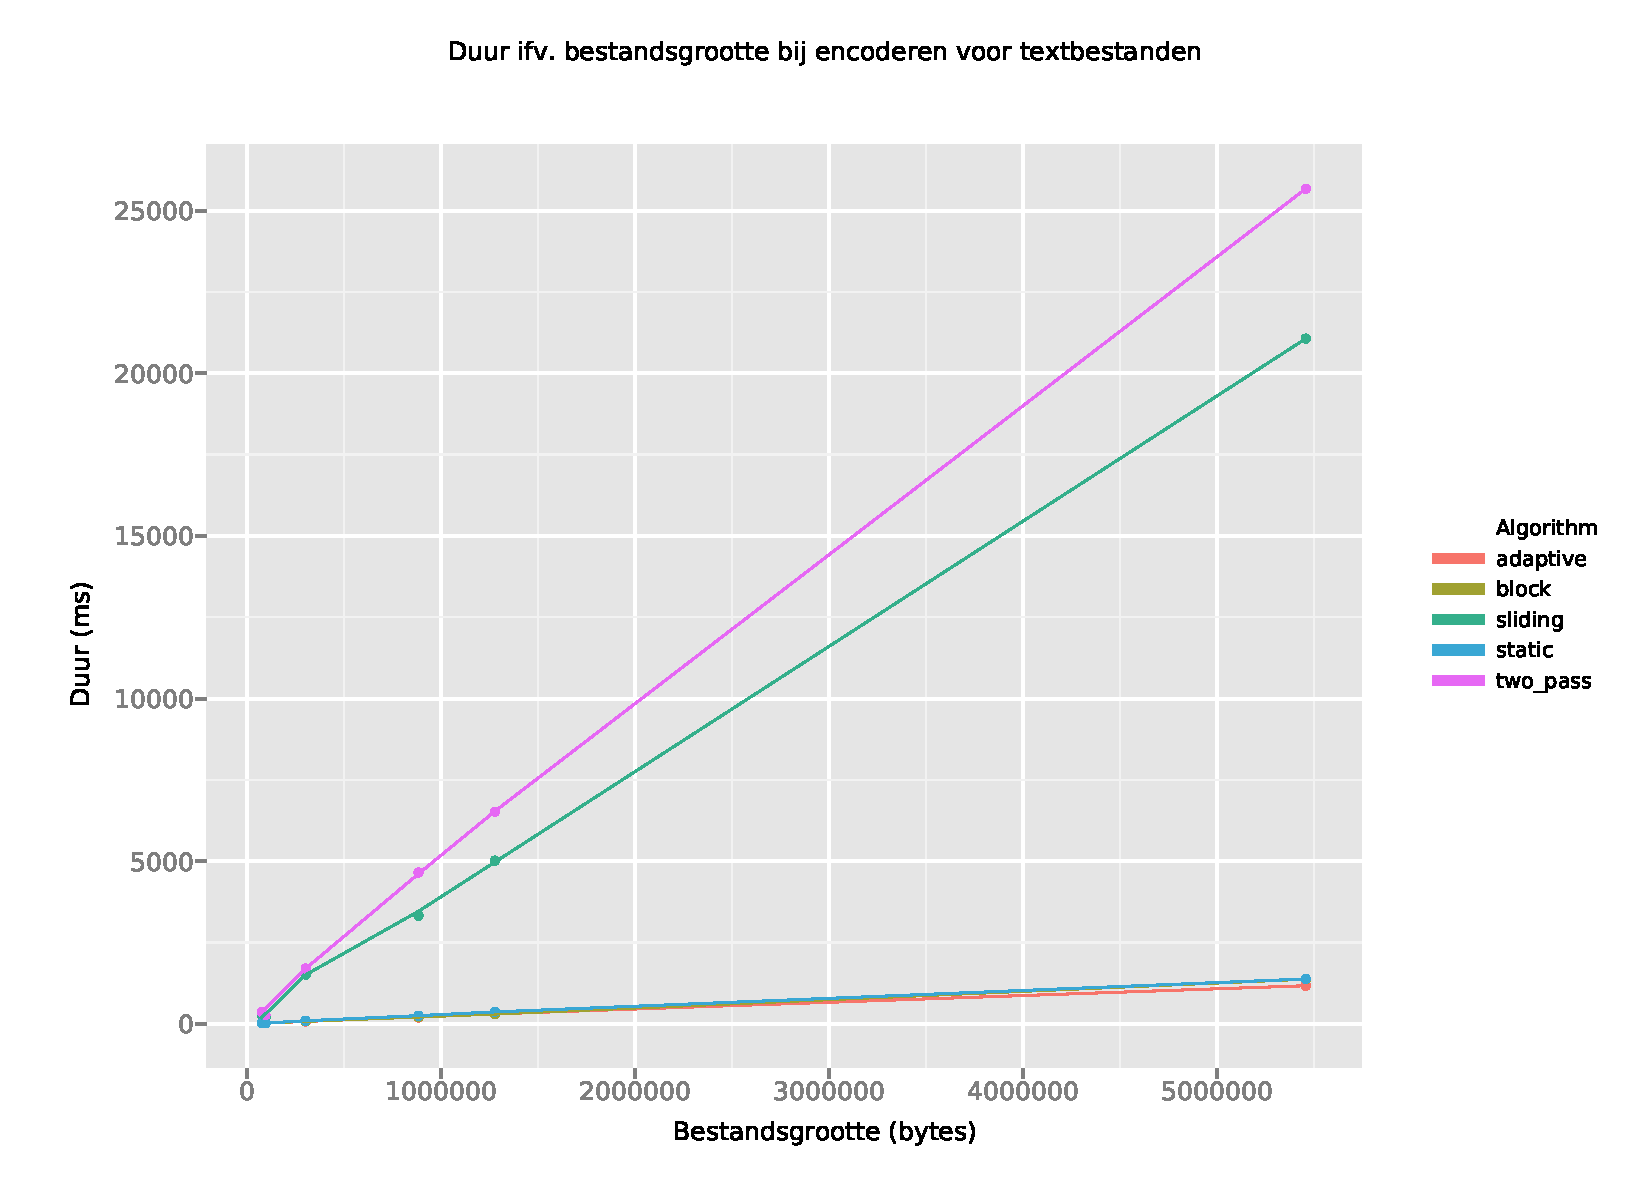
\includegraphics[width=.5\linewidth]{../experimenten/grafieken/duur/encode_textbestanden.pdf}\hfil
%		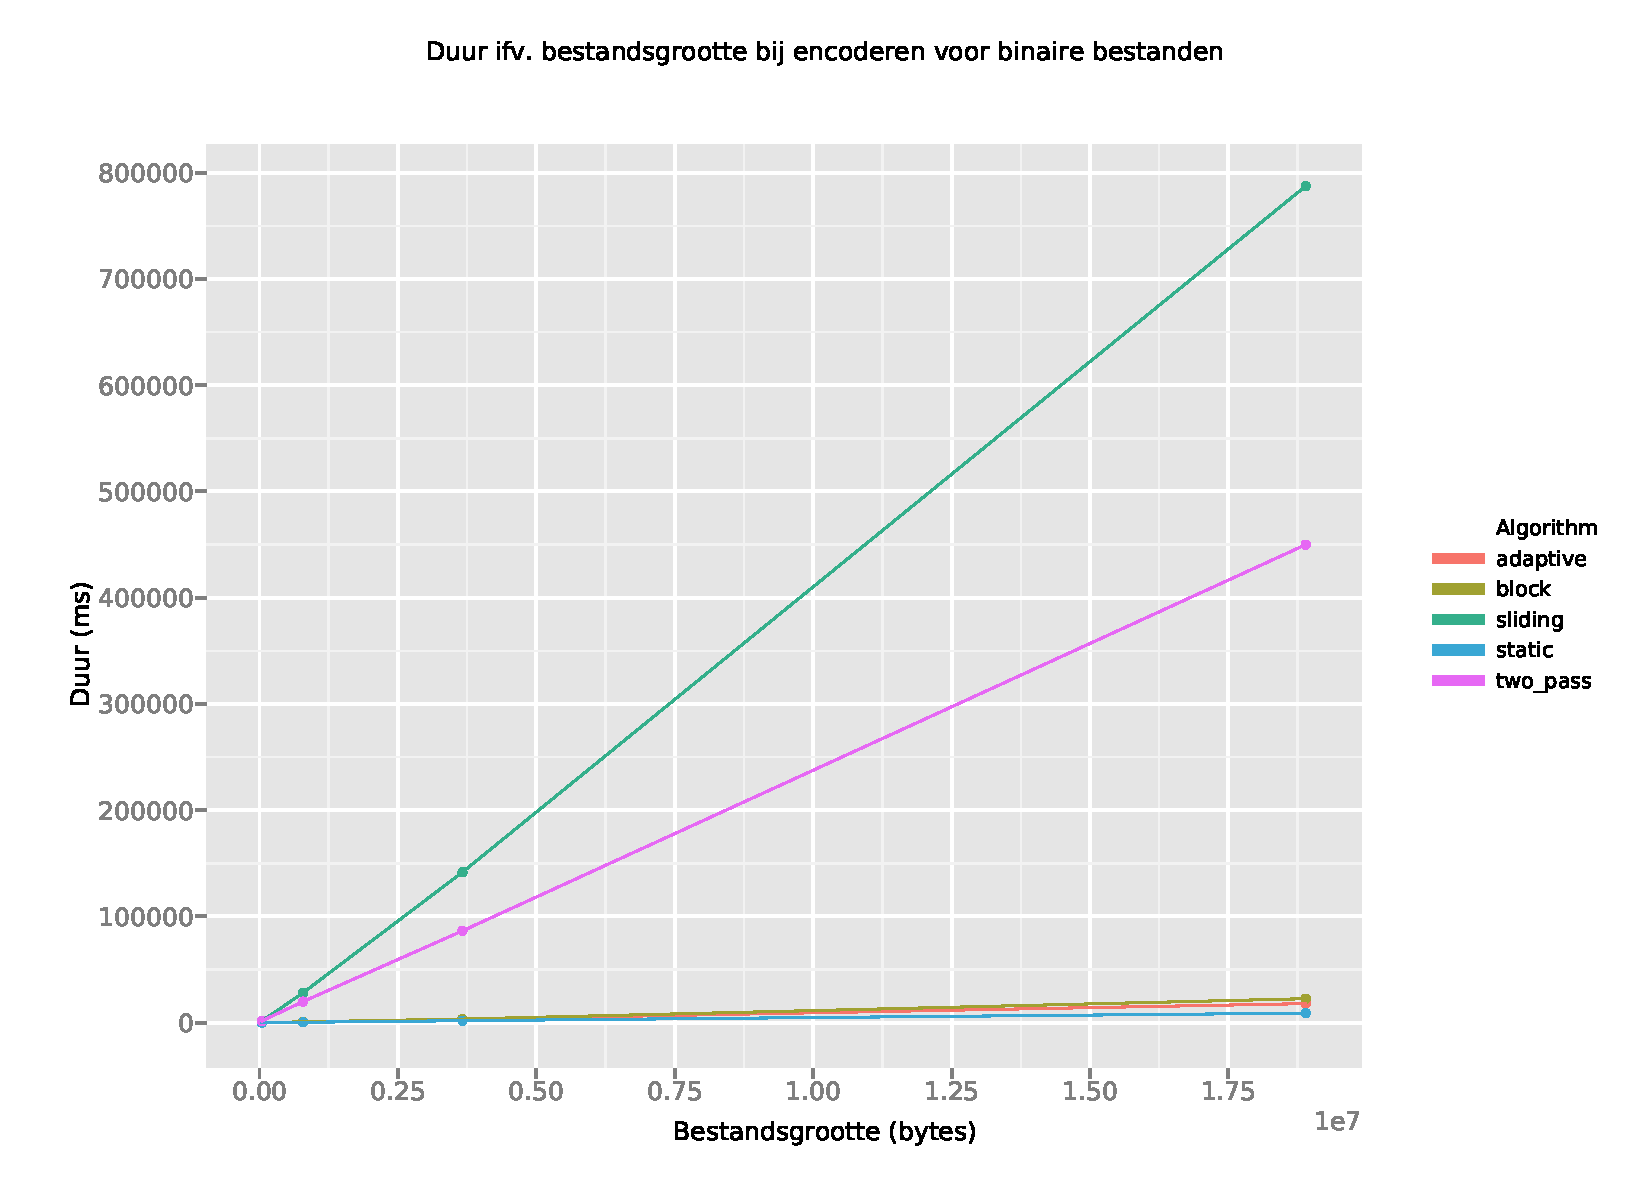
\includegraphics[width=.5\linewidth]{../experimenten/grafieken/duur/encode_binaire_bestanden.pdf}
%	\end{subfigure}
%	\begin{subfigure}{\linewidth}
%		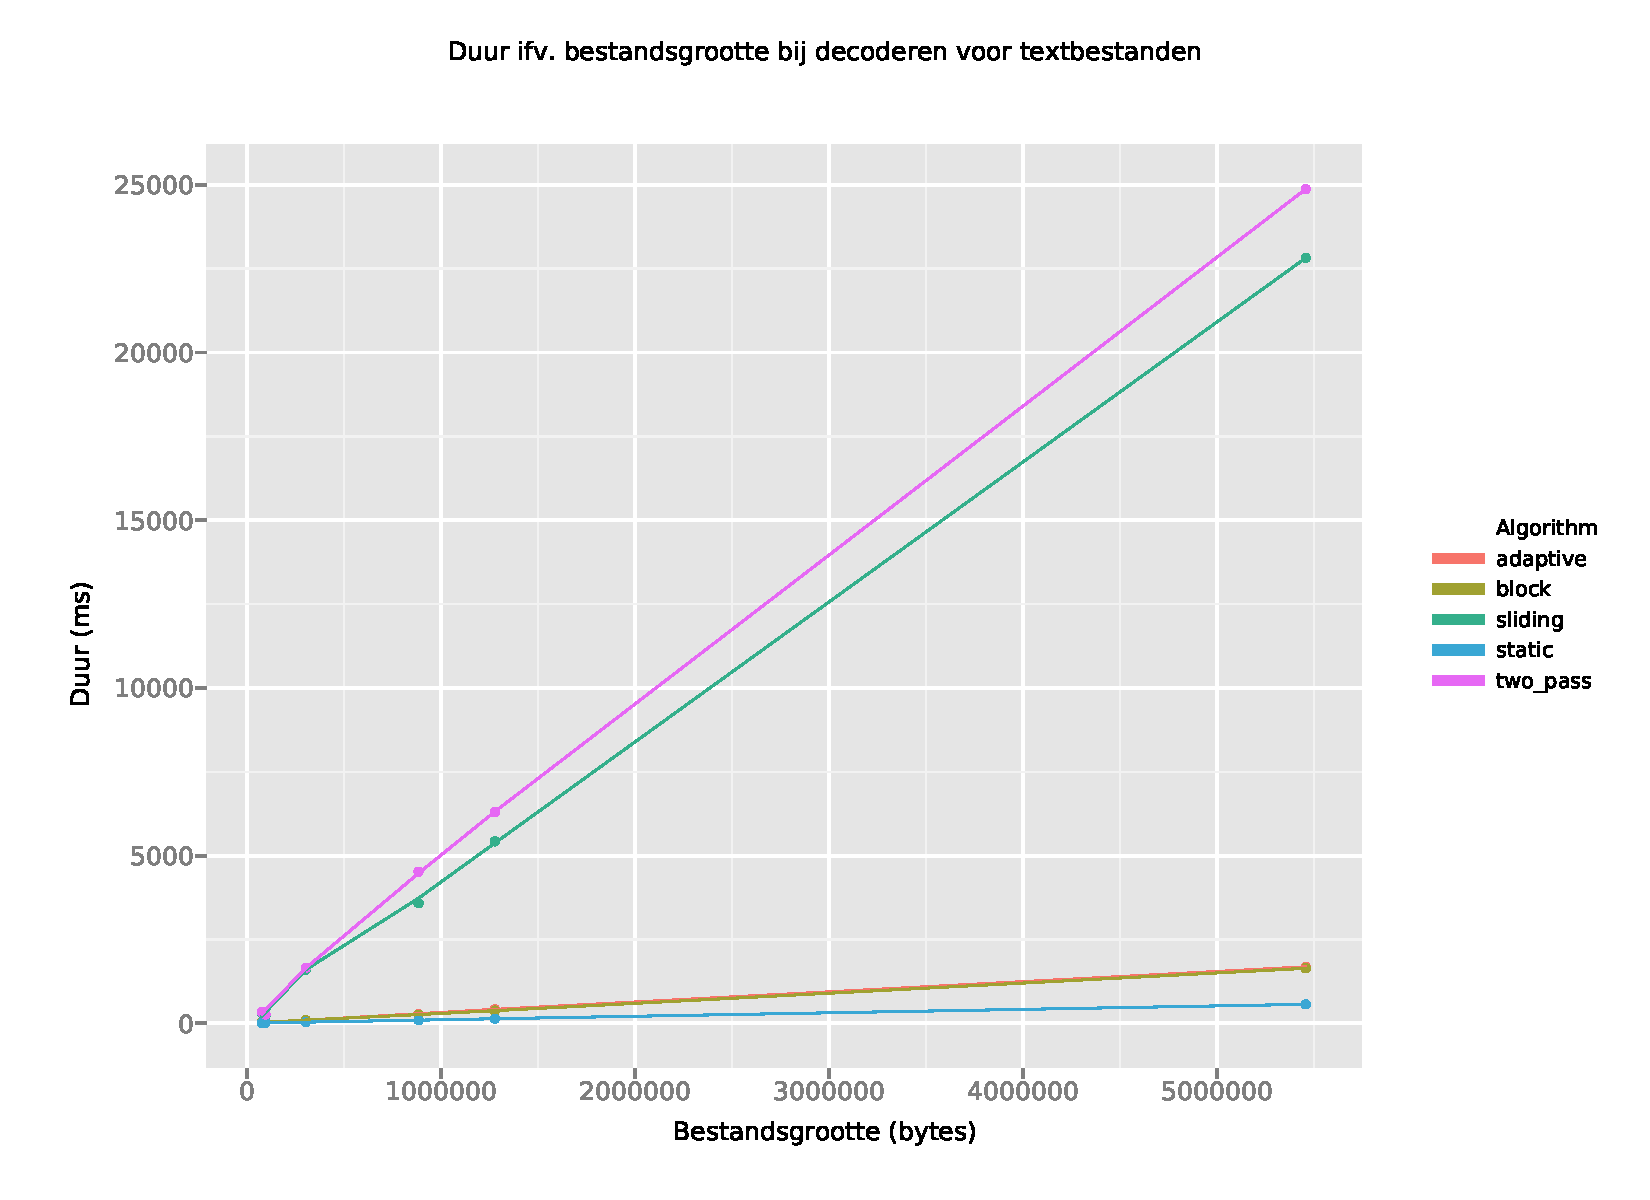
\includegraphics[width=.5\linewidth]{../experimenten/grafieken/duur/decode_textbestanden.pdf}\hfil
%		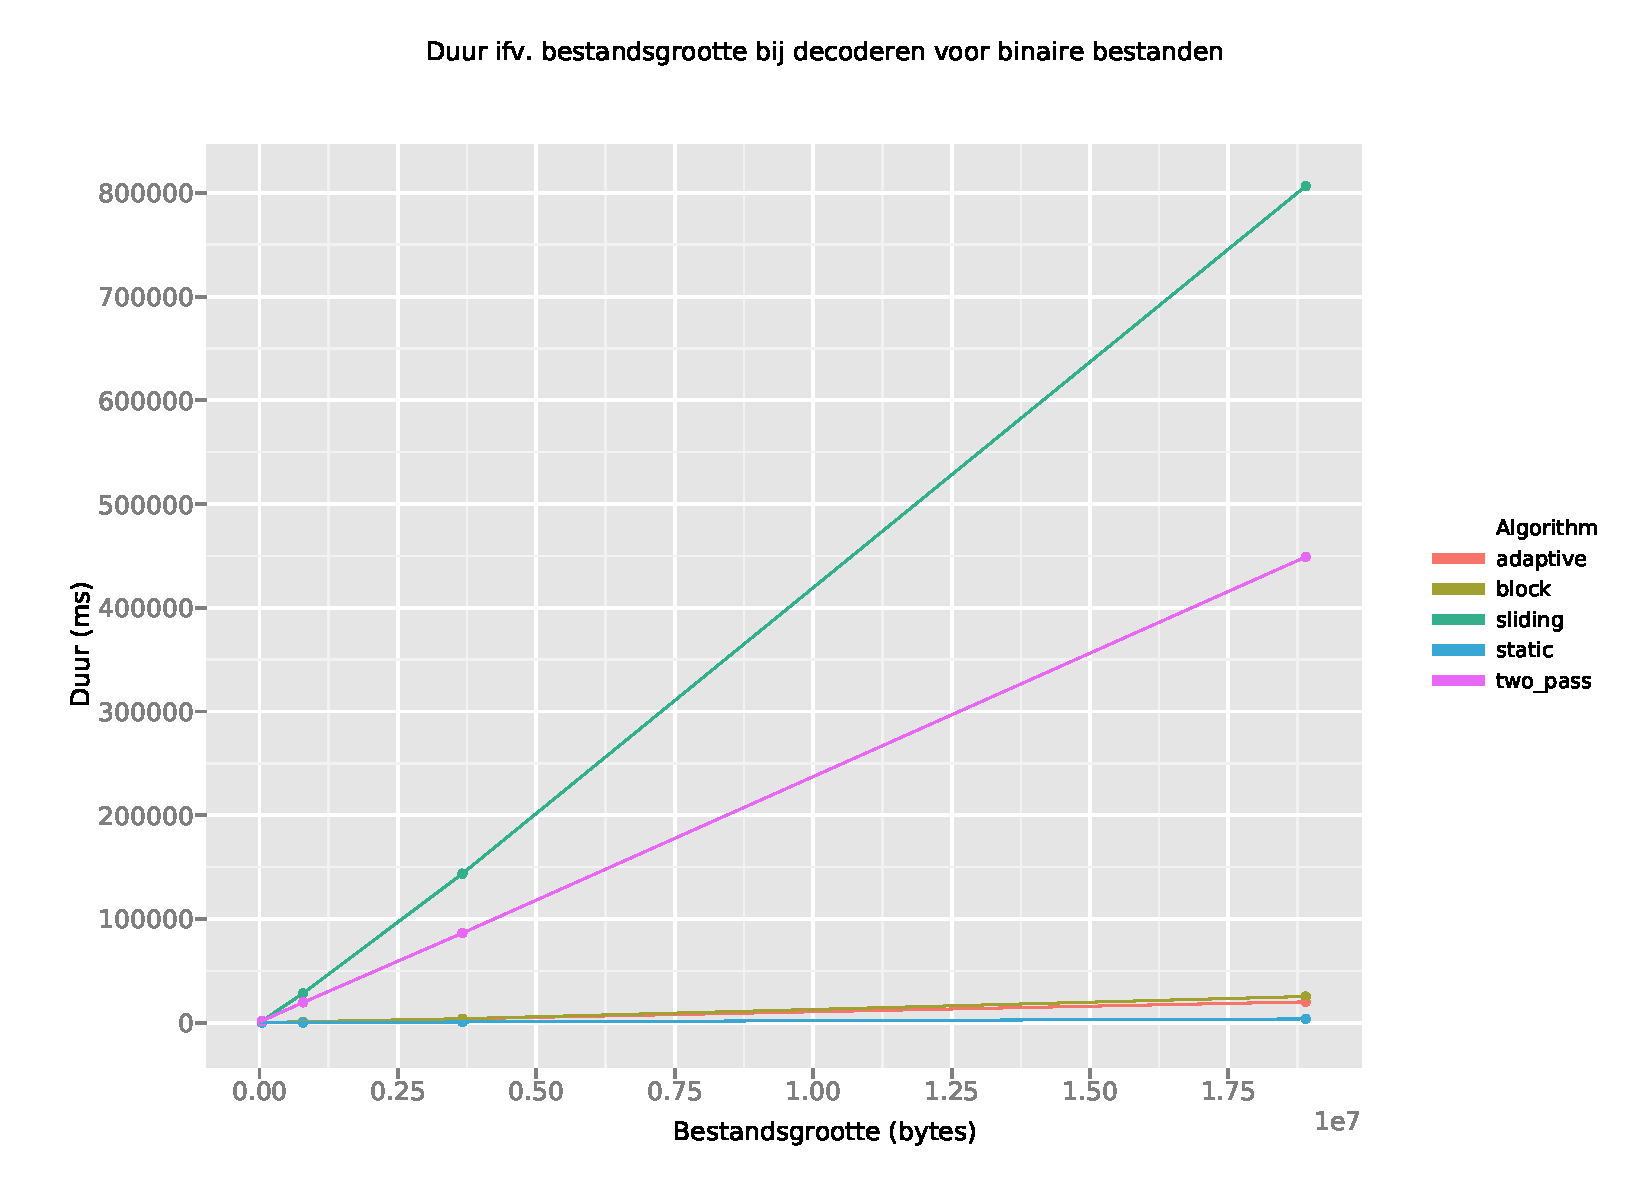
\includegraphics[width=.5\linewidth]{../experimenten/grafieken/duur/decode_binaire_bestanden.pdf}
%	\end{subfigure}
%\end{figure}

\chapter{Besluit}
%%%%%Statisch
\section{Statische huffman}

%%%%%Adaptive huffman
\section{Adaptive huffman}


%%%%%%%%Adaptive huffman met sliding window
\section{Adaptive huffman met sliding window}

%%%%%Two pass
\section{Two pass adaptive huffman}

%%%%%Blocksgewijze adaptive huffman
\section{Bloksgewijze adaptive huffman}

%%%%%Bloksgewijze adaptive huffman
\end{document}